\documentclass[8pt]{beamer}

\newif\ifplacelogo % create a new conditional
\placelogotrue % set it to true

\usetheme{Warsaw}
\usecolortheme{rose}
\usepackage{multicol}
\usepackage{epstopdf}
\usepackage[italic]{hepnames}
\usepackage{tikz}
\usepackage{listings}
\usepackage{times}
\usepackage{amsmath}
\usepackage{verbatim}
\usepackage{hyperref}
\usepackage{bbding}
\usepackage{gensymb}
\usepackage{upgreek}
\lstset{breakatwhitespace,
language=C++,
columns=fullflexible,
keepspaces,
breaklines,
tabsize=3, 
showstringspaces=false,
extendedchars=true}

% TikZ includes!!!
\usepackage{tikz}
\usetikzlibrary{backgrounds}
\usetikzlibrary{calc}
\tikzstyle{every picture}+=[remember picture]
\input{/home/oviazlo/Desktop/beamerPresentations/myReports/latexHelpScripts/tikzGrid.tex}


\begin{document}

% custom colors
\definecolor{olive}{rgb}{0.3, 0.4, .1}
\definecolor{fore}{RGB}{249,242,215}
\definecolor{back}{RGB}{51,51,51}
\definecolor{title}{RGB}{255,0,90}
\definecolor{dgreen}{rgb}{0.,0.6,0.}
\definecolor{gold}{rgb}{1.,0.84,0.}
\definecolor{JungleGreen}{cmyk}{0.99,0,0.52,0}
\definecolor{BlueGreen}{cmyk}{0.85,0,0.33,0}
\definecolor{RawSienna}{cmyk}{0,0.72,1,0.45}
\definecolor{Magenta}{cmyk}{0,1,0,0}

\definecolor{PixelColor}{RGB}{207,232,139}
\definecolor{SCTColor}{RGB}{167,166,255}
\definecolor{TRTColor}{RGB}{250,224,140}
\definecolor{grayColor}{RGB}{153,153,153}

\newcommand{\yRefPosOne}{0.0}
\newcommand{\xRefPosOne}{0.0}
\newcommand{\yRefPosTwo}{0.0}
\newcommand{\xRefPosTwo}{0.0}
\newcommand{\yRefIncrementOne}{0.0}
\newcommand{\xRefIncrementOne}{0.0}
\newcommand{\yRefIncrementTwo}{0.0}
\newcommand{\xRefIncrementTwo}{0.0}

\graphicspath{ {/home/oviazlo/Desktop/beamerPresentations/FCCee/pictures/CALOR2018/} }


\DeclareGraphicsExtensions{.eps, .pdf, .png}

\newcommand{\myBox}[2][pink] {
    \noindent\colorbox{#1}{
	\textbf{#2}
    }\par
}

% For nice block (provided by Oleh)
\tikzstyle{myBox} = [draw=red, fill=blue!1, very thick,
    rectangle, rounded corners, inner sep=5pt, inner ysep=9pt]
    
\tikzstyle{PixelBox} = [draw=PixelColor, fill=blue!1, very thick,
    rectangle, rounded corners, inner sep=5pt, inner ysep=9pt]
\tikzstyle{SCTBox} = [draw=SCTColor, fill=blue!1, very thick,
    rectangle, rounded corners, inner sep=5pt, inner ysep=9pt]
\tikzstyle{TRTBox} = [draw=TRTColor, fill=blue!1, very thick,
    rectangle, rounded corners, inner sep=5pt, inner ysep=9pt]

% poster advertisement
\newcommand{\myCenterBox}[2][pink] {
   {\centering
    \noindent\colorbox{#1}{
	\textbf{#2}
    }\par
  }
}

\newcommand{\mySmallCenterBox}[2][pink] {
   {\centering
    \noindent\colorbox{#1}{
	\textbf{{\small #2}}
    }\par
  }
}

\newcommand{\myVerySmallCenterBox}[2][pink] {
   {\centering
    \noindent\colorbox{#1}{
	\textbf{{\scriptsize #2}}
    }\par
  }
}

\newcommand{\backupbegin}{
   \newcounter{finalframe}
   \setcounter{finalframe}{\value{framenumber}}
}
\newcommand{\backupend}{
   \setcounter{framenumber}{\value{finalframe}}
}

\newcommand{\myNode}{\tikz[baseline,inner sep=1pt] \node[anchor=base]}

\tikzstyle{fancytitle} =[fill=white!15, text=black]

\definecolor{light-gray}{gray}{0.95}
% poster advertisement


\title[Software compensation \hspace{19.0em}\insertframenumber/
\inserttotalframenumber]{ Software compensation }


	\author[Oleksandr Viazlo]{Oleksandr Viazlo\\ 
	{\small }
	}
	\institute{\small CERN\\} 
	
       
	\date{29 May 2018}

% 	\logo{ \ifplacelogo \includegraphics[height=1.8cm]{./ID_week2/lund_uni-logo_s.pdf} \hspace{0.4cm} \fi}

	
%    	\frame{\titlepage}

   	

\placelogofalse


%*****************************************************************************
\begin{frame}{\large \large Software Compensation}
\renewcommand{\yRefPosOne}{0}
\renewcommand{\xRefPosOne}{5.3}
\renewcommand{\xRefIncrementOne}{5.5}

 \begin{tikzpicture}[overlay]
 
%   \node[inner sep=0pt] (tmp) at (\xRefPosOne,\yRefPosOne+0.5)
%     {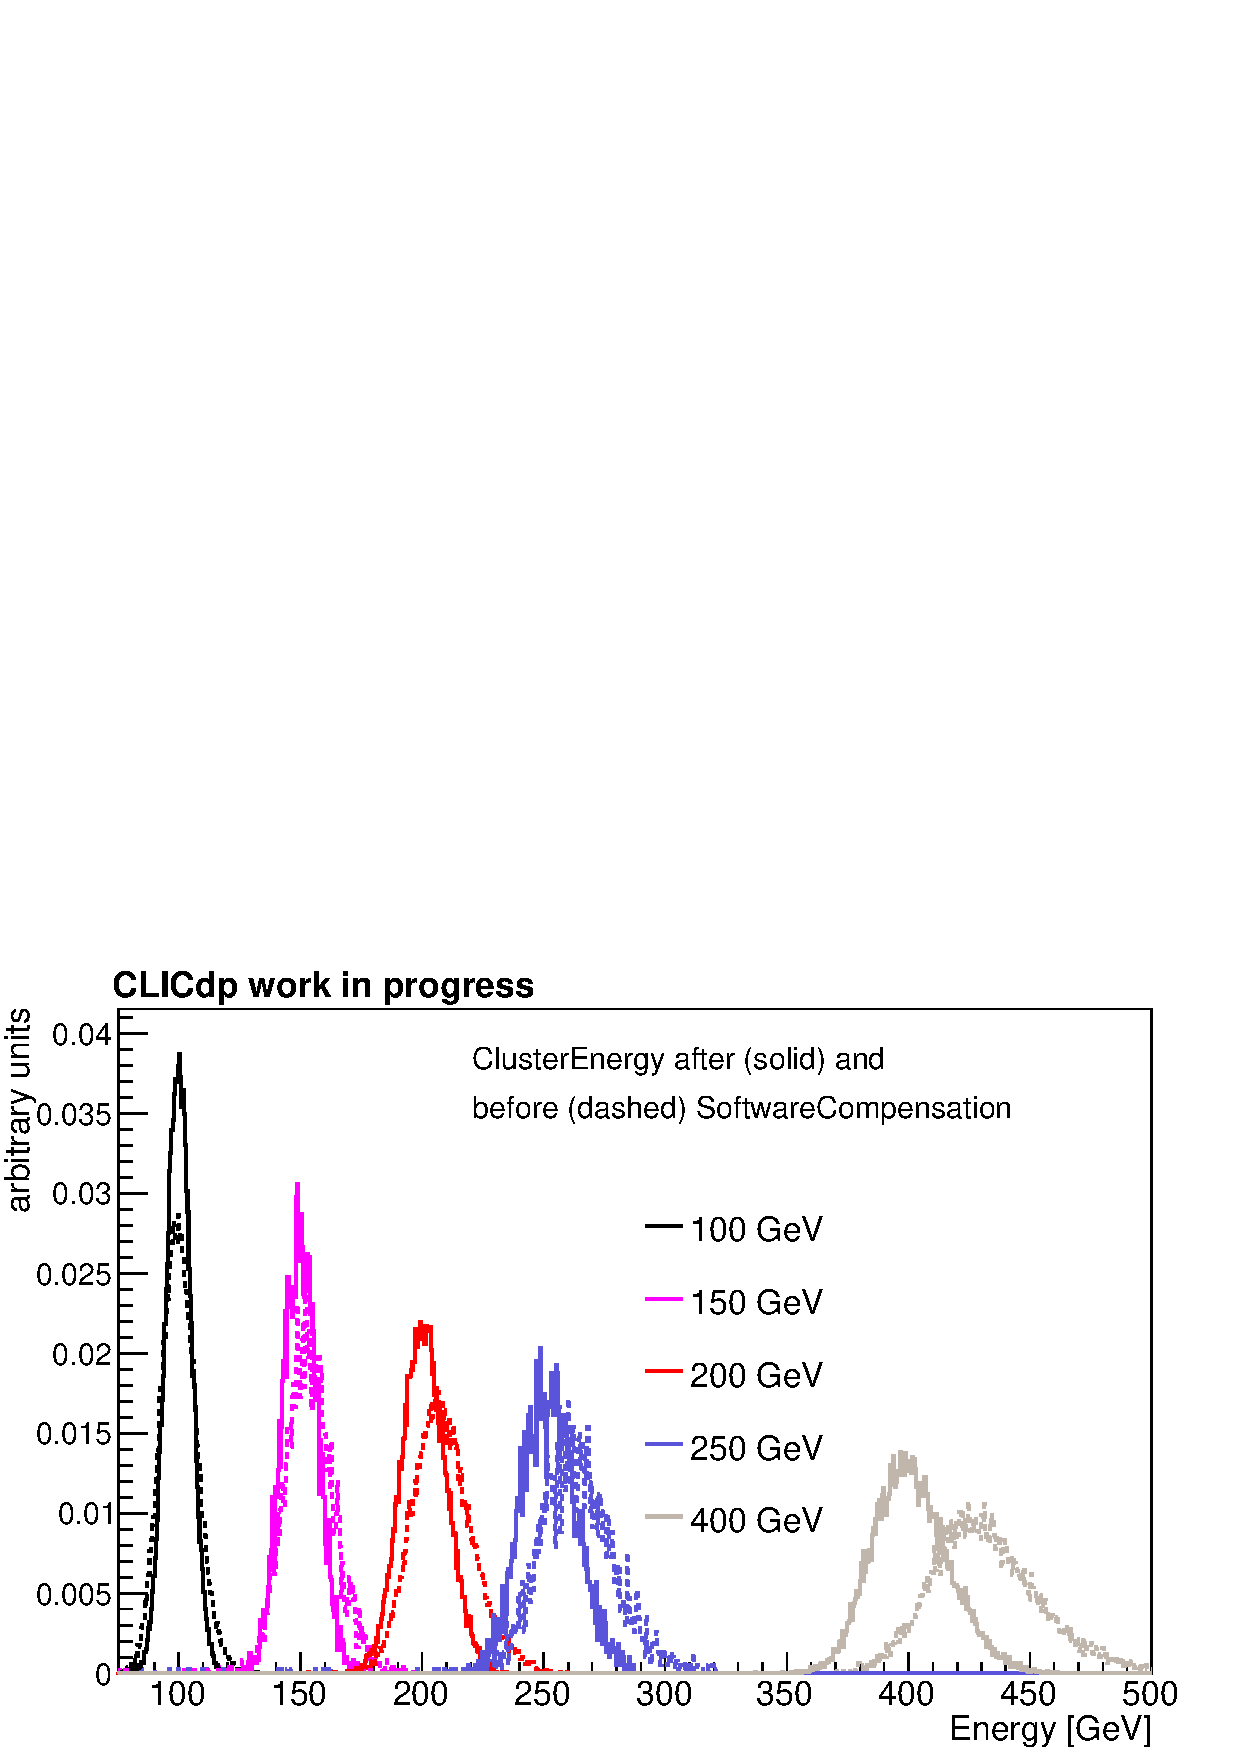
\includegraphics[width=8cm]{Matthias/ClosurePlotOfHighEnergyRangeNeutrons.pdf}};

 \node[inner sep=0pt] (tmp) at (\xRefPosOne+3.5,\yRefPosOne-2.0)
    {\includegraphics[width=5cm]{fromPreviousTalks/swComp_weights_example.png}};
 
 
 
 \node  at (\xRefPosOne-2.7,\yRefPosOne-1.8) (box){%
    \begin{minipage}{0.6\textwidth}
    Software compensation:
  \begin{itemize}
   \item Electromagnetic component of shower typically denser
   \item Software compensation reweights hits in HCAL depending on the hit energy
density
    \item Weights are calculated by formula: $\omega(\rho) = $p$_1 $exp$($p$_2 \rho) + $p$_3$ \\[0.1cm]
    where each parameter is an energy dependent\\ $\to$
    9 different parameters are used in total
    
%    \item In total 9 different parameters are used
%    \item Weight includes an energy dependence
   
  \end{itemize}
    \end{minipage}
};

\node  at (\xRefPosOne-0.6,\yRefPosOne+1.8) (box){%
    \begin{minipage}{1.05\textwidth}
%     Nonlinear non compensating natures of hadron calorimeters:
  \begin{itemize}
    \item Software compensation is an energy ``regularisation'' techniques ({\small  \href{http://iopscience.iop.org/1748-0221/7/09/P09017}{\color{blue}JINST 7 (2012) P09017}})
   \item Idea is to correct with software for (on average) larger response of hadron
showers with large electromagnetic component $\to$ improves energy
measurement of cluster energies
   \item Software compensation technique (developed by CALICE) is implemented in
PandoraPFA now
  \end{itemize}
    \end{minipage}
};

\node [PixelBox] at (\xRefPosOne-2.3,\yRefPosOne-4.2) (box){%
  \begin{minipage}{0.55\textwidth}
  Detector specific software compensation weights were obtained for CLICdet and CLD 
  \end{minipage}
};

% \node [PixelBox] at (\xRefPosOne,\yRefPosOne-4) (box){%
%   \begin{minipage}{\textwidth}
%   Default weight tuned for ILD experiment at ILC up to 100 GeV, at CLIC expect to
% reach higher hadron energies, at 3 TeV sometimes beyond 500 GeV
% $\to$ retune parameters for CLIC ({\small Follow description of paper EPJC 77 (2017) 698})
%   \end{minipage}
% };

\node  at (\xRefPosOne+4.95,\yRefPosOne+0.63) (box){%
\myVerySmallCenterBox[TRTColor]{EPJC 77 (2017) 698}
}; 





\end{tikzpicture}
 
\end{frame}
%*****************************************************************************
%*****************************************************************************
\begin{frame}{\large \large Software compensation for CLD, CLICdet and ILD}
\renewcommand{\yRefPosOne}{-1.5}
\renewcommand{\xRefPosOne}{4.2}
\renewcommand{\xRefIncrementOne}{7.5}
\begin{tikzpicture}[overlay]

 \node[inner sep=0pt] (tmp) at (\xRefPosOne-1.7,\yRefPosOne+2.9)
  {\includegraphics[width=4cm]{../newSW_may29/may29_SWC_weights_1_GeV.pdf}};
  \node  at (\xRefPosOne-1.7,\yRefPosOne+4.5) (box){%
\myCenterBox{\small 1 GeV}
}; 
  
 \node[inner sep=0pt] (tmp) at (\xRefPosOne+4.5,\yRefPosOne+2.9)
  {\includegraphics[width=4cm]{../newSW_may29/may29_SWC_weights_5_GeV.pdf}};
  \node  at (\xRefPosOne+4.5,\yRefPosOne+4.5) (box){%
\myCenterBox{\small 5 GeV}
}; 

 \node[inner sep=0pt] (tmp) at (\xRefPosOne-2.9,\yRefPosOne-0.9)
  {\includegraphics[width=4cm]{../newSW_may29/may29_SWC_weights_10_GeV.pdf}};
  \node  at (\xRefPosOne-2.9,\yRefPosOne+0.7) (box){%
\myCenterBox{\small 10 GeV}
}; 
  
   \node[inner sep=0pt] (tmp) at (\xRefPosOne+1.1,\yRefPosOne-0.9)
  {\includegraphics[width=4cm]{../newSW_may29/may29_SWC_weights_30_GeV.pdf}};
    \node  at (\xRefPosOne+1.1,\yRefPosOne+0.7) (box){%
\myCenterBox{\small 30 GeV}
}; 
  
 \node[inner sep=0pt] (tmp) at (\xRefPosOne+4.9,\yRefPosOne-0.9)
  {\includegraphics[width=4cm]{../newSW_may29/may29_SWC_weights_90_GeV.pdf}};
  \node  at (\xRefPosOne+4.9,\yRefPosOne+0.7) (box){%
\myCenterBox{\small 90 GeV}
}; 
 
  
 
 
 

  
\end{tikzpicture}
\end{frame}
%*****************************************************************************
%*****************************************************************************
\begin{frame}{\large \large Jet energy resolution with dijet events}

\renewcommand{\yRefPosOne}{-1.5}
\renewcommand{\xRefPosOne}{5.3}
\renewcommand{\xRefIncrementOne}{5.5}
\begin{tikzpicture}[overlay]

  \node  at (\xRefPosOne+0.4,\yRefPosOne+4.5) (box){%
    \begin{minipage}{1.1\textwidth}
  \begin{itemize}
  \item Dijet events of a Z-like particle decaying into pair of light quarks (u, d, s) at several centre-of-mass energies
    \end{itemize}
    \end{minipage}
  };

 \node[inner sep=0pt] (tmp) at (\xRefPosOne-2.7,\yRefPosOne+1.2)
    {\includegraphics[width=6cm]{JER_FCCee_vs_CLIC_conformal_Zuds91_matthiasCLIC.pdf}};
    
 \node[inner sep=0pt] (tmp) at (\xRefPosOne+3.3,\yRefPosOne+1.2)
    {\includegraphics[width=6cm]{JER_FCCee_vs_CLIC_conformal_Zuds380_matthiasCLIC.pdf}};
    
 \node[inner sep=0pt] (tmp) at (\xRefPosOne-3.6,\yRefPosOne+3.5)
    {\tiny WORK IN PROGRESS};
 \node[inner sep=0pt] (tmp) at (\xRefPosOne+2.4,\yRefPosOne+3.5)
    {\tiny WORK IN PROGRESS};
    
\node  at (\xRefPosOne-1.13,\yRefPosOne+3.55) (box){%
\myCenterBox{\small 45.5 GeV jets}
}; 

\node  at (\xRefPosOne+4.9,\yRefPosOne+3.55) (box){%
\myCenterBox{\small 190 GeV jets}
}; 



\node  at (\xRefPosOne,\yRefPosOne-2.3) (box){%
\begin{minipage}{\textwidth}
  \begin{itemize}
   \item Comparable resolution for both detectors
    \item Jet energy resolution in barrel region:
    \begin{itemize}
        \item 45.5 GeV jets: 4-5 $\%$
        \item 190 GeV jets: 3-4 $\%$ \\ [0.2cm]
    \end{itemize}
  \end{itemize}
\end{minipage}
};

  \node [PixelBox, inner sep=4pt]  at (\xRefPosOne+3.55,\yRefPosOne-2.4) (box){%
    \begin{minipage}{0.45\textwidth}
    \small
		Jet energy (E$_j$) is measured as a half of total energy (E$_{jj}$) of Z$\to q\bar{q}$ (q=u,d,s) di-jet event\\
		
		\hspace{0.4cm}
		  {\includegraphics[width=4cm]{../plots_FCCweek_workshop/other/jetRes_formula.png}}
		
    \end{minipage}
  };

% % HELPER draw advanced helping grid with axises:
% \draw(-0.5,-4) to[grid with coordinates] (11.5,4);
\end{tikzpicture}
 
\end{frame}
%*****************************************************************************

\end{document}

